% =====================================================================
%  Major Project Presentation (Beamer): Mock Interview AI
%  Compile with pdfLaTeX (Overleaf default). Overleaf runs it twice
%  automatically, which the title-slide background needs.
% =====================================================================
\documentclass[aspectratio=169,11pt,xcolor=table]{beamer}

% ---------------------------------------------------------------------
%  EDIT THIS BLOCK: your details
% ---------------------------------------------------------------------
\newcommand{\projecttitle}{Mock Interview AI}
\newcommand{\projectsubtitle}{An AI-Powered Mock Interview Platform with CV Analysis, Voice Interaction and Behavioural Feedback}
\newcommand{\studentlines}{STUDENT NAME 1 (Roll No.: XXXXXXXX)\\ STUDENT NAME 2 (Roll No.: XXXXXXXX)\\ STUDENT NAME 3 (Roll No.: XXXXXXXX)}
\newcommand{\teamshort}{Team}
\newcommand{\guideline}{Under the guidance of GUIDE NAME, Assistant Professor}
\newcommand{\collegeline}{Department of Computer Science and Engineering\\ COLLEGE NAME, UNIVERSITY NAME}
\newcommand{\collegeshort}{COLLEGE NAME}
\newcommand{\presentationdate}{MONTH YEAR}
% ---------------------------------------------------------------------

\usepackage[utf8]{inputenc}
\usepackage[T1]{fontenc}
\usepackage{lmodern}
\usepackage{booktabs}
\usepackage{tabularx}
\usepackage{array}
\usepackage{amsmath}
\usepackage{tikz}
\usetikzlibrary{positioning,arrows.meta,shapes.geometric,calc}

% ---------- theme and colours (the app's palette) ----------
\usetheme{Madrid}
\definecolor{coral}{RGB}{220,78,78}
\definecolor{brandmagenta}{RGB}{176,52,164}
\definecolor{brandamber}{RGB}{214,138,24}
\definecolor{brandcyan}{RGB}{16,150,178}
\definecolor{ink}{RGB}{34,26,60}
\setbeamercolor{palette primary}{bg=ink,fg=white}
\setbeamercolor{palette secondary}{bg=brandmagenta,fg=white}
\setbeamercolor{palette tertiary}{bg=coral,fg=white}
\setbeamercolor{palette quaternary}{bg=ink,fg=white}
\setbeamercolor{frametitle}{bg=ink,fg=white}
\setbeamercolor{title}{bg=ink,fg=white}
\setbeamercolor{structure}{fg=coral}
\setbeamercolor{block title}{bg=coral,fg=white}
\setbeamercolor{block body}{bg=coral!7,fg=black}
\setbeamercolor{block title example}{bg=brandcyan,fg=white}
\setbeamercolor{block body example}{bg=brandcyan!7,fg=black}
\setbeamercolor{block title alerted}{bg=brandamber,fg=white}
\setbeamercolor{block body alerted}{bg=brandamber!8,fg=black}
\setbeamertemplate{navigation symbols}{}
\setbeamertemplate{itemize items}[circle]
\setbeamertemplate{enumerate items}[default]
\setbeamertemplate{blocks}[rounded][shadow=false]
\setbeamertemplate{caption}{\raggedright\insertcaption\par}
\setbeamerfont{frametitle}{series=\bfseries}
\newcolumntype{Y}{>{\raggedright\arraybackslash}X}

\title[\projecttitle]{\projecttitle}
\subtitle{\projectsubtitle}
\author[\teamshort]{\studentlines}
\institute[\collegeshort]{\collegeline}
\date{\presentationdate}

% ---------- diagram styles ----------
\tikzset{
  box/.style={draw=ink!70, rounded corners=3pt, fill=#1, align=center, minimum height=0.9cm, text width=2.5cm, font=\scriptsize},
  box/.default={coral!10},
  flow/.style={draw=ink!70, rounded corners=3pt, fill=#1, align=center, minimum height=1.1cm, text width=1.6cm, font=\scriptsize},
  flow/.default={coral!10},
  arrow/.style={-{Stealth[length=2mm]}, thick, draw=ink!70},
  biarrow/.style={{Stealth[length=2mm]}-{Stealth[length=2mm]}, thick, draw=ink!70},
  lbl/.style={font=\tiny, fill=white, inner sep=1pt, align=center},
  st/.style={draw=ink!70, circle, fill=#1, minimum size=1.5cm, font=\scriptsize\bfseries, align=center},
  st/.default={coral!12}
}
\setbeamertemplate{bibliography item}[text]

\begin{document}

% =====================================================================
%  TITLE
% =====================================================================
\begin{frame}[plain]
  
\begin{tikzpicture}[remember picture, overlay]
    \shade[left color=ink, right color=brandmagenta!70!ink] (current page.south west) rectangle (current page.north east);
    \fill[coral, opacity=0.25] ([xshift=-1.5cm,yshift=-1cm]current page.north east) circle (3cm);
    \fill[brandamber, opacity=0.18] ([xshift=1cm,yshift=1cm]current page.south west) circle (2.5cm);
  \end{tikzpicture}
  \vspace{0.4cm}
  \begin{center}
    {\color{brandamber}\footnotesize\bfseries MAJOR PROJECT PRESENTATION\par}
    \vspace{0.25cm}
    {\color{white}\Huge\bfseries \projecttitle\par}
    \vspace{0.2cm}
    {\color{white!85!coral}\normalsize \projectsubtitle\par}
    \vspace{0.6cm}
    {\color{white}\small \studentlines\par}
    \vspace{0.35cm}
    {\color{white!80}\footnotesize \guideline\par}
    \vspace{0.2cm}
    {\color{white!80}\footnotesize \collegeline\par}
    \vspace{0.15cm}
    {\color{white!70}\scriptsize \presentationdate\par}
  \end{center}
\end{frame}

% =====================================================================
\begin{frame}{Outline}
  \begin{columns}[T]
    \begin{column}{0.48\textwidth}
      \begin{enumerate}
        \item Introduction and problem statement
        \item Objectives
        \item Literature survey and research gap
        \item Proposed system
        \item Architecture and workflow
        \item CV analysis and question generation
        \item Interview room: speech and code
      \end{enumerate}
    \end{column}
    \begin{column}{0.48\textwidth}
      \begin{enumerate}\setcounter{enumi}{7}
        \item Computer vision for body language
        \item Resilient AI access and Offline mode
        \item Final report
        \item Implementation and technology stack
        \item Testing and results
        \item Limitations and future scope
        \item Conclusion
      \end{enumerate}
    \end{column}
  \end{columns}
\end{frame}

% =====================================================================
\section{Introduction}
\begin{frame}{Introduction}
  \begin{itemize}
    \item Interviews decide careers: a \textbf{technical round} (projects, fundamentals, coding) and an \textbf{HR round} (communication, motivation, fit).
    \item Candidates practise by reading question lists and solving problems \emph{silently}, which is very different from a real interview.
    \item Real interviewers:
      \begin{itemize}
        \item ask \textbf{about your CV} first,
        \item want answers \textbf{spoken aloud}, with follow-ups,
        \item notice \textbf{body language} such as eye contact and nervousness.
      \end{itemize}
    \item Human mock interviews help, but need an expert, time and scheduling, and rarely give structured feedback.
  \end{itemize}
\end{frame}

\begin{frame}{Problem Statement}
  \begin{block}{Problem}
    Design and implement a cross-platform application that conducts a realistic, \textbf{voice-based} mock interview \textbf{personalised to the candidate's CV}, academic record and experience level, with a technical round of \textbf{at most 90 minutes} and a separate \textbf{HR round of at most 15 minutes}, that analyses answers, code and on-camera behaviour, and produces a detailed performance and CV report.
  \end{block}
  \vspace{0.3cm}
  \begin{itemize}
    \item Must run on \textbf{Windows and macOS}.
    \item Must stay usable when the AI service is busy or unavailable.
  \end{itemize}
\end{frame}

\begin{frame}{Objectives}
  \begin{enumerate}
    \item Collect the academic record (10th, 12th / Diploma, UG, PG, PhD: stream and score) and the CV; \textbf{analyse the CV}.
    \item Offer three levels: \textbf{Beginner} (fresher), \textbf{Intermediate} (2--3 years), \textbf{Hard} (8+ years).
    \item Generate questions, about \textbf{65\% from the CV}, plus \textbf{FAANG coding problems} for software roles.
    \item \textbf{Speak} questions, \textbf{transcribe} answers, provide a \textbf{code editor}.
    \item Analyse the \textbf{webcam on the device}: eye contact, presence, extra faces, expressions.
    \item Enforce time limits: technical $\le 90$ min, HR $\le 15$ min.
    \item Produce a \textbf{detailed report} with model answers and a CV review, downloadable as \textbf{PDF}.
  \end{enumerate}
\end{frame}

% =====================================================================
\section{Literature Survey}
\begin{frame}{Literature Survey}
  \small
  \begin{tabularx}{\textwidth}{@{}p{3.6cm}Y@{}}
    \toprule
    \textbf{Work} & \textbf{Key idea and relevance} \\
    \midrule
    Campion et al.\ 1997; Levashina et al.\ 2014 & Structured interviews (planned questions, defined scoring) are more reliable. We plan every question with expected key points. \\
    Hoque et al.\ 2013 (MACH) & Virtual agent for mock interviews with speech and face feedback improved performance. No CV-based questions. \\
    Naim et al.\ 2018 & Verbal, prosodic and facial features predict interview ratings (speaking rate, fewer fillers, smiling). \\
    Lugaresi et al.\ 2019; Kartynnik et al.\ 2019 & MediaPipe: real-time 3D face landmarks on web and mobile. Basis of our vision module. \\
    Gemini Team 2023; Zheng et al.\ 2023 & Multimodal LLMs read PDFs; LLM-as-judge agrees well with humans on open answers. \\
    \bottomrule
  \end{tabularx}
\end{frame}

\begin{frame}{Existing Approaches and Research Gap}
  \footnotesize
  \begin{tabularx}{\textwidth}{@{}Ycccccc@{}}
    \toprule
    \textbf{Approach} & \textbf{CV} & \textbf{Voice} & \textbf{Camera} & \textbf{Coding} & \textbf{HR} & \textbf{Report} \\
    \midrule
    Question lists and books & -- & -- & -- & partly & partly & -- \\
    Coding practice websites & -- & -- & -- & yes & -- & partly \\
    Peer mock-interview platforms & partly & yes & yes & yes & partly & partly \\
    Generic AI practice tools & -- & partly & -- & -- & partly & partly \\
    Research prototypes & -- & yes & yes & -- & yes & partly \\
    \rowcolor{coral!12}\textbf{Proposed system} & \textbf{yes} & \textbf{yes} & \textbf{yes} & \textbf{yes} & \textbf{yes} & \textbf{yes} \\
    \bottomrule
  \end{tabularx}
  \vspace{0.3cm}
  \begin{alertblock}{Gap}
    No single free tool combines CV-driven questions, spoken interaction, real coding problems, on-device behaviour analysis, separate timed rounds and a combined performance and CV report.
  \end{alertblock}
\end{frame}

% =====================================================================
\section{Proposed System}
\begin{frame}{Proposed System: Mock Interview AI}
  \begin{columns}[T]
    \begin{column}{0.5\textwidth}
      \small
      \begin{itemize}
        \item Browser-based: Chrome / Edge on \textbf{Windows and macOS}
        \item CV analysis with scores and red flags
        \item Three difficulty levels
        \item CV-based and FAANG questions
        \item Spoken questions, live transcript, code editor
        \item On-device body-language analysis
        \item Technical round then separate HR round
        \item Detailed report and PDF
        \item Works with or without an AI key
      \end{itemize}
    \end{column}
    \begin{column}{0.48\textwidth}
      \centering
      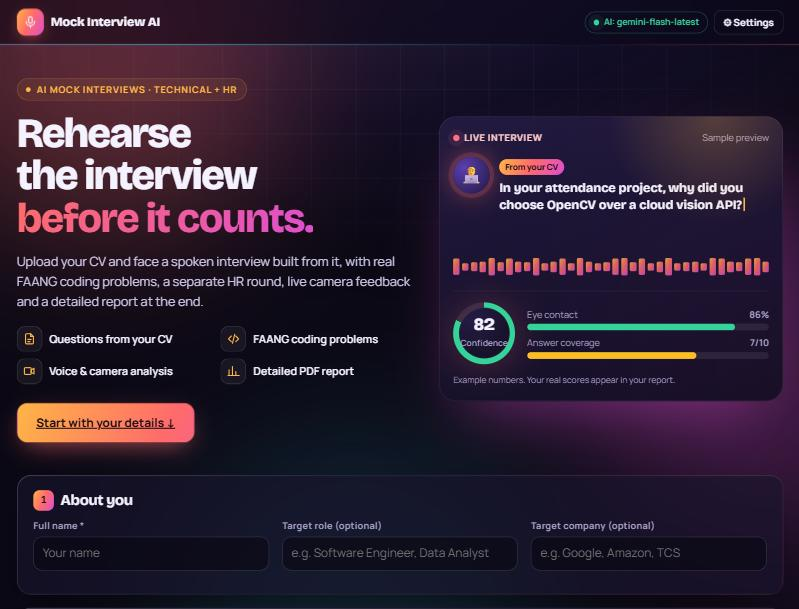
\includegraphics[width=\linewidth,height=0.75\textheight,keepaspectratio]{figures/landing_hero.jpg}
    \end{column}
  \end{columns}
\end{frame}

\begin{frame}{System Architecture}
  \centering
  \resizebox{0.95\textwidth}{!}{%
  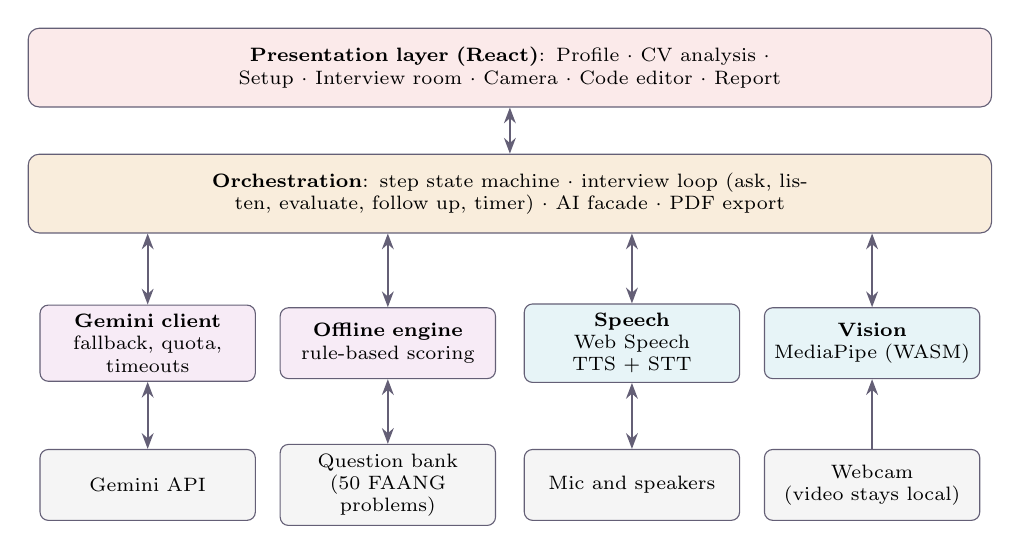
\begin{tikzpicture}
    \node[draw=ink!70, rounded corners=4pt, fill=coral!12, text width=12cm, align=center, minimum height=1cm, font=\scriptsize] (ui) at (0,0) {\textbf{Presentation layer (React)}: Profile $\cdot$ CV analysis $\cdot$ Setup $\cdot$ Interview room $\cdot$ Camera $\cdot$ Code editor $\cdot$ Report};
    \node[draw=ink!70, rounded corners=4pt, fill=brandamber!15, text width=12cm, align=center, minimum height=1cm, font=\scriptsize] (orch) at (0,-1.6) {\textbf{Orchestration}: step state machine $\cdot$ interview loop (ask, listen, evaluate, follow up, timer) $\cdot$ AI facade $\cdot$ PDF export};
    \node[box={brandmagenta!10}] (gem) at (-4.6,-3.5) {\textbf{Gemini client}\\ fallback, quota, timeouts};
    \node[box={brandmagenta!10}] (off) at (-1.55,-3.5) {\textbf{Offline engine}\\ rule-based scoring};
    \node[box={brandcyan!10}] (sp) at (1.55,-3.5) {\textbf{Speech}\\ Web Speech TTS + STT};
    \node[box={brandcyan!10}] (vis) at (4.6,-3.5) {\textbf{Vision}\\ MediaPipe (WASM)};
    \node[box={gray!8}] (api) at (-4.6,-5.3) {Gemini API};
    \node[box={gray!8}] (bank) at (-1.55,-5.3) {Question bank\\ (50 FAANG problems)};
    \node[box={gray!8}] (dev) at (1.55,-5.3) {Mic and speakers};
    \node[box={gray!8}] (cam) at (4.6,-5.3) {Webcam\\ (video stays local)};
    \draw[biarrow] (ui) -- (orch);
    \foreach \n in {gem,off,sp,vis} \draw[biarrow] (orch.south -| \n.north) -- (\n.north);
    \draw[biarrow] (gem) -- (api);
    \draw[biarrow] (off) -- (bank);
    \draw[biarrow] (sp) -- (dev);
    \draw[arrow] (cam) -- (vis);
  \end{tikzpicture}}
\end{frame}

\begin{frame}{Workflow}
  \centering
  \resizebox{\textwidth}{!}{%
  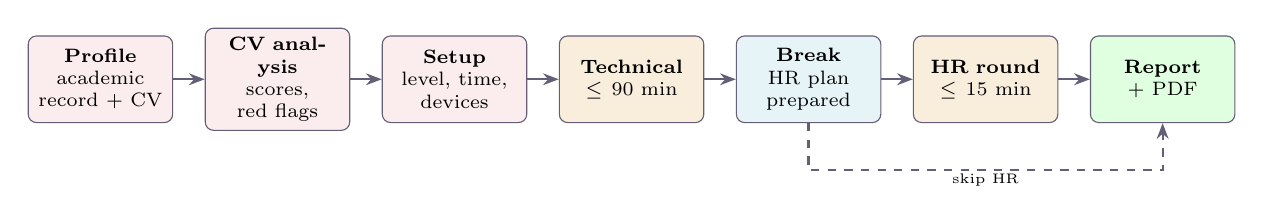
\begin{tikzpicture}
    \node[flow] (a) at (0,0) {\textbf{Profile}\\ academic record + CV};
    \node[flow, right=0.4cm of a] (b) {\textbf{CV analysis}\\ scores, red flags};
    \node[flow, right=0.4cm of b] (c) {\textbf{Setup}\\ level, time, devices};
    \node[flow={brandamber!15}, right=0.4cm of c] (d) {\textbf{Technical}\\ $\le 90$ min};
    \node[flow={brandcyan!10}, right=0.4cm of d] (e) {\textbf{Break}\\ HR plan prepared};
    \node[flow={brandamber!15}, right=0.4cm of e] (f) {\textbf{HR round}\\ $\le 15$ min};
    \node[flow={green!12}, right=0.4cm of f] (g) {\textbf{Report}\\ + PDF};
    \draw[arrow] (a) -- (b);
    \draw[arrow] (b) -- (c);
    \draw[arrow] (c) -- (d);
    \draw[arrow] (d) -- (e);
    \draw[arrow] (e) -- (f);
    \draw[arrow] (f) -- (g);
    \draw[arrow, dashed] (e.south) -- ++(0,-0.6) -| node[lbl, pos=0.25, below] {skip HR} (g.south);
  \end{tikzpicture}}
  \vspace{0.5cm}
  \begin{itemize}
    \small
    \item The order is fixed, like a real interview process.
    \item Each round ends automatically when its timer expires; it can end earlier if all questions are done.
  \end{itemize}
\end{frame}

% =====================================================================
\section{Core Modules}
\begin{frame}{CV Analysis}
  \begin{columns}[T]
    \begin{column}{0.44\textwidth}
      \small
      \begin{itemize}
        \item PDF and images read \textbf{directly by Gemini}; DOCX via mammoth; text as-is.
        \item Six scores: overall, ATS, clarity, impact, formatting, relevance.
        \item Skills, projects, experience, strengths, weaknesses.
        \item \textbf{Red flags} interviewers will probe, e.g.\ a \textbf{92\% $\to$ 74\%} dip from 10th to 12th.
        \item Suggested level from estimated experience.
        \item CGPA converted: $9.5 \times g$ (out of 10), $25 \times g$ (out of 4).
      \end{itemize}
    \end{column}
    \begin{column}{0.54\textwidth}
      \centering
      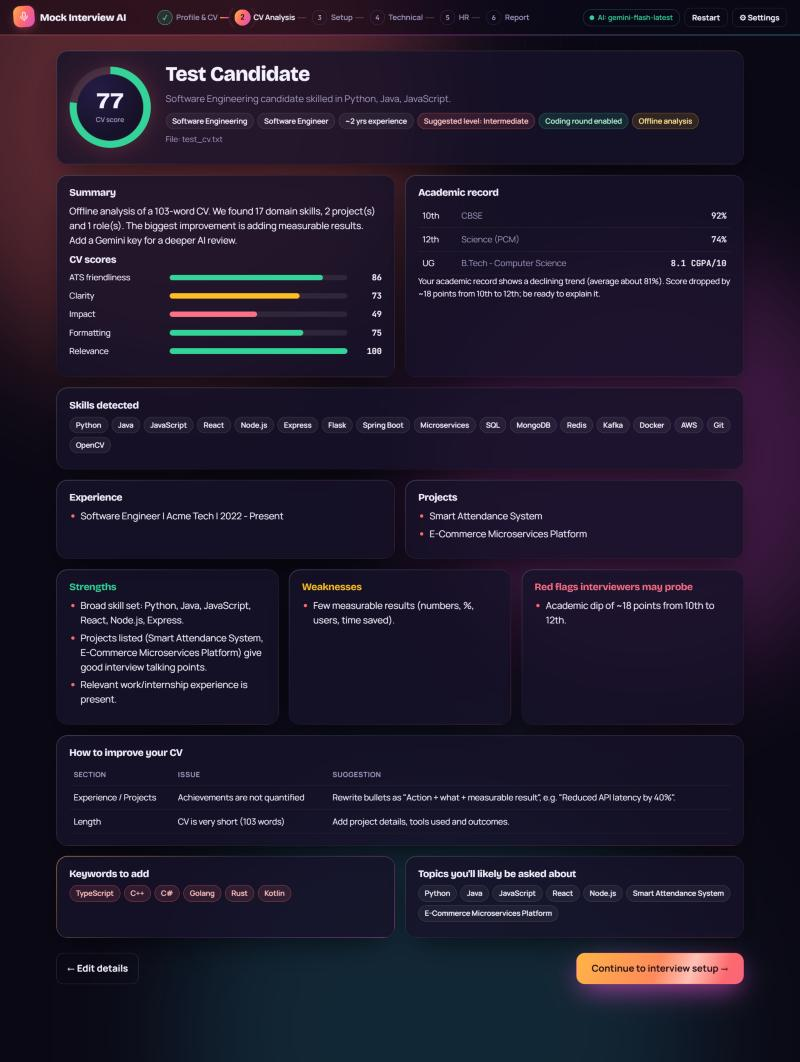
\includegraphics[width=\linewidth,height=0.78\textheight,keepaspectratio]{figures/cv_analysis.jpg}
    \end{column}
  \end{columns}
\end{frame}

\begin{frame}{Question Generation}
  \small
  \begin{itemize}
    \item About \textbf{65\% of questions name a specific CV item} (project, internship, skill); the rest cover fundamentals at the chosen level.
    \item First question: warm-up on the candidate's most relevant project.
    \item Number of coding ($n_c$) and design ($n_d$) problems for a round of $T$ minutes:
  \end{itemize}
  \[
    n_c = \begin{cases} 0 & \text{not a software role}\\ 1 & T < 25\\ 2 & 25 \le T \le 60\\ 3 & T > 60 \end{cases}
    \qquad
    n_d = \begin{cases} 1 & \text{software, level} \ne \text{Beginner}, T \ge 30\\ 0 & \text{otherwise} \end{cases}
  \]
  \begin{itemize}
    \item Suggested times must add up to between $0.8T$ and $T$.
    \item Coding problems drawn from a bank of \textbf{50 FAANG-reported problems} (16 easy, 22 medium, 12 hard), tagged with the companies known to ask them.
    \item HR round: 3 / 5 / 7 questions for 5 / 10 / 15 min; asks about CV red flags; ends with ``Do you have any questions for us?''
  \end{itemize}
\end{frame}

\begin{frame}{Interview Room}
  \begin{columns}[T]
    \begin{column}{0.46\textwidth}
      \small
      \begin{itemize}
        \item Question \textbf{spoken aloud} (text-to-speech), shown word by word.
        \item Answer \textbf{transcribed live} (speech recognition); can also type or edit.
        \item \textbf{Monaco code editor} for coding questions (Python, Java, C++, JavaScript, C, Go).
        \item Each answer evaluated; natural \textbf{follow-up} if the answer is vague (max 4 technical, 2 HR).
        \item Timer is a hard limit; no new coding problem with $< 8$ min left.
      \end{itemize}
    \end{column}
    \begin{column}{0.52\textwidth}
      \centering
      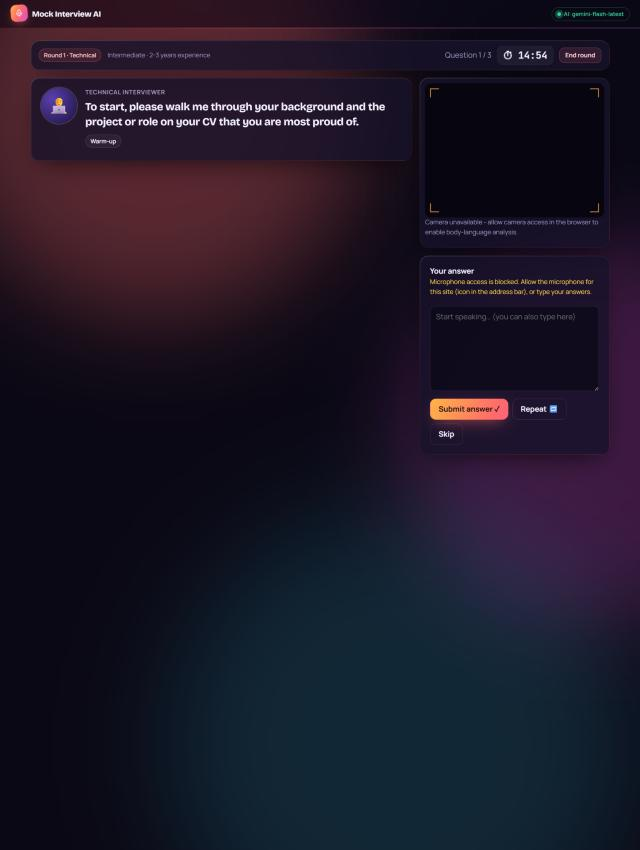
\includegraphics[width=\linewidth,height=0.78\textheight,keepaspectratio]{figures/interview_room.jpg}
    \end{column}
  \end{columns}
\end{frame}

\begin{frame}{Interview State Machine and Speech Processing}
  \begin{columns}[T]
    \begin{column}{0.52\textwidth}
      \centering
      \resizebox{\linewidth}{!}{%
      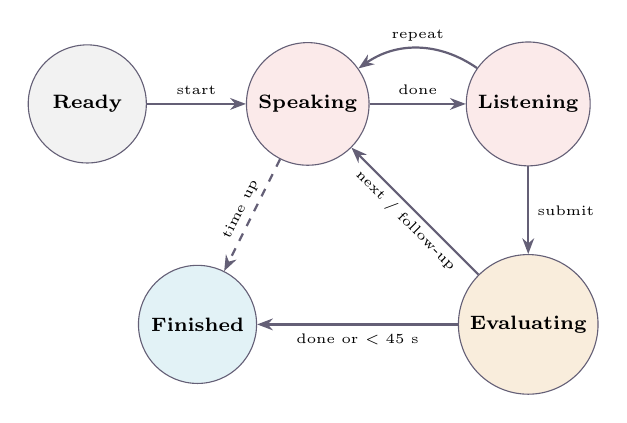
\begin{tikzpicture}
        \node[st={gray!10}] (r) at (0,0) {Ready};
        \node[st={coral!12}] (s) at (2.8,0) {Speaking};
        \node[st={coral!12}] (l) at (5.6,0) {Listening};
        \node[st={brandamber!15}] (e) at (5.6,-2.8) {Evaluating};
        \node[st={brandcyan!12}] (f) at (1.4,-2.8) {Finished};
        \draw[arrow] (r) -- node[lbl, above=2pt] {start} (s);
        \draw[arrow] (s) -- node[lbl, above=2pt] {done} (l);
        \draw[arrow] (l) to[bend right=35] node[lbl, above=1pt] {repeat} (s);
        \draw[arrow] (l) -- node[lbl, right=2pt] {submit} (e);
        \draw[arrow] (e) -- node[lbl, sloped, below=1pt] {next / follow-up} (s);
        \draw[arrow] (e) -- node[lbl, below=2pt] {done or $<45$ s} (f);
        \draw[arrow, dashed] (s) -- node[lbl, sloped, above=1pt] {time up} (f);
      \end{tikzpicture}}
    \end{column}
    \begin{column}{0.46\textwidth}
      \small
      \begin{itemize}
        \item Long questions split into $\le 180$-character chunks (browsers cut long speech).
        \item Recognition paused while the interviewer speaks (no echo).
        \item Auto-restart after silences; interim words kept.
        \item Metrics: words, \textbf{WPM} $= N_{\text{words}} / (t/60)$, 13 filler words (``um'', ``basically'', ``you know'').
      \end{itemize}
    \end{column}
  \end{columns}
\end{frame}

\begin{frame}{Computer Vision: Body-Language Analysis}
  \small
  \begin{itemize}
    \item \textbf{MediaPipe Face Landmarker} in the browser (WebAssembly, GPU): \textbf{478 landmarks + 52 blendshapes}, $\approx$10 frames/s, up to 3 faces. \textbf{Video never leaves the device.}
    \item Head orientation from landmarks (nose 1, cheeks 234 / 454, forehead 10, chin 152):
  \end{itemize}
  \[
    r_{\text{yaw}} = \frac{x_{1} - x_{234}}{x_{454} - x_{234}}, \qquad r_{\text{pitch}} = \frac{y_{1} - y_{10}}{y_{152} - y_{10}}
  \]
  \begin{itemize}
    \item \textbf{Calibrated} to the candidate over the first 20 frontal frames; away if $|\Delta r_{\text{yaw}}| > 0.14$ or $|\Delta r_{\text{pitch}}| > 0.10$, or gaze blendshapes $> 0.55$.
    \item Also: face present, extra faces, smile ($>0.35$), tension ($>0.45$), blinks, head movement. Gaze paused while coding.
  \end{itemize}
  \begin{block}{Estimated confidence score (\%)}
    \centering
    $C = 0.40\,E + 0.20\,F + 0.15\,(100 - T) + 0.10\,M + 0.15\min(100, 4S)$
  \end{block}
\end{frame}

\begin{frame}{Resilient AI Access}
  \small
  \textbf{Problem found:} free Gemini tier $\approx$ \textbf{20 requests / model / day}, frequent \textbf{503 ``high demand''}, a model hanging for 2 min, and the original model \textbf{retired} for new keys.
  \vspace{0.3cm}

  \centering
  \resizebox{\textwidth}{!}{%
  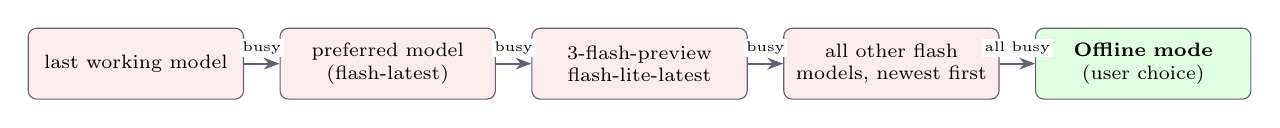
\begin{tikzpicture}
    \node[box] (m1) at (0,0) {last working model};
    \node[box, right=0.45cm of m1] (m2) {preferred model\\ (flash-latest)};
    \node[box, right=0.45cm of m2] (m3) {3-flash-preview\\ flash-lite-latest};
    \node[box, right=0.45cm of m3] (m4) {all other flash models, newest first};
    \node[box={green!12}, right=0.45cm of m4] (off) {\textbf{Offline mode}\\ (user choice)};
    \draw[arrow] (m1) -- node[lbl, above=2pt] {busy} (m2);
    \draw[arrow] (m2) -- node[lbl, above=2pt] {busy} (m3);
    \draw[arrow] (m3) -- node[lbl, above=2pt] {busy} (m4);
    \draw[arrow] (m4) -- node[lbl, above=2pt] {all busy} (off);
  \end{tikzpicture}}
  \vspace{0.3cm}

  \raggedright
  \begin{itemize}
    \item 404 $\to$ model marked \textbf{retired}; 429 daily quota $\to$ \textbf{exhausted}; both skipped for the session.
    \item 429 / 5xx $\to$ next model; network error or bad JSON $\to$ one retry.
    \item Per-request timeout and overall budget: 60 / 75 s (planning), \textbf{20 / 30 s (live grading, then local scoring)}, 90 / 180 s (report).
  \end{itemize}
\end{frame}

\begin{frame}{Offline Mode: Works Without Any Key}
  \small
  \begin{itemize}
    \item \textbf{CV}: section detection, $\approx$160 skills in 9 domains, experience from year ranges, six rule-based scores, e.g.
      \[ \text{Impact} = \operatorname{clamp}_{[5,100]}\bigl(20 + 10q + 3\min(a,15) - 4w\bigr) \]
      ($q$: measurable results, $a$: action verbs, $w$: weak phrases).
    \item \textbf{Questions}: templates from CV projects, roles and skills + question bank.
    \item \textbf{Answers}: key-point coverage $c$, length $\ell$, structure $s$:
      \[ \text{score}_{\text{verbal}} = 10\,(0.55\,c + 0.30\,\ell + 0.15\,s) \]
    \item \textbf{Verdict} from weighted overall score: Strong Hire $\ge 85$, Hire $\ge 72$, Lean Hire $\ge 60$, Lean No Hire $\ge 45$.
    \item All offline results are labelled as \textbf{estimates}.
  \end{itemize}
\end{frame}

\begin{frame}{Final Report}
  \begin{columns}[T]
    \begin{column}{0.44\textwidth}
      \small
      \begin{itemize}
        \item Overall score and \textbf{hire verdict}.
        \item 7 category scores: technical, problem solving, coding, communication, HR, body language, CV alignment.
        \item Every question: your answer, feedback, \textbf{model answer}.
        \item Communication and body-language tips.
        \item \textbf{CV review}: did answers back up the CV?
        \item Personal \textbf{study plan}; \textbf{PDF} download.
      \end{itemize}
    \end{column}
    \begin{column}{0.54\textwidth}
      \centering
      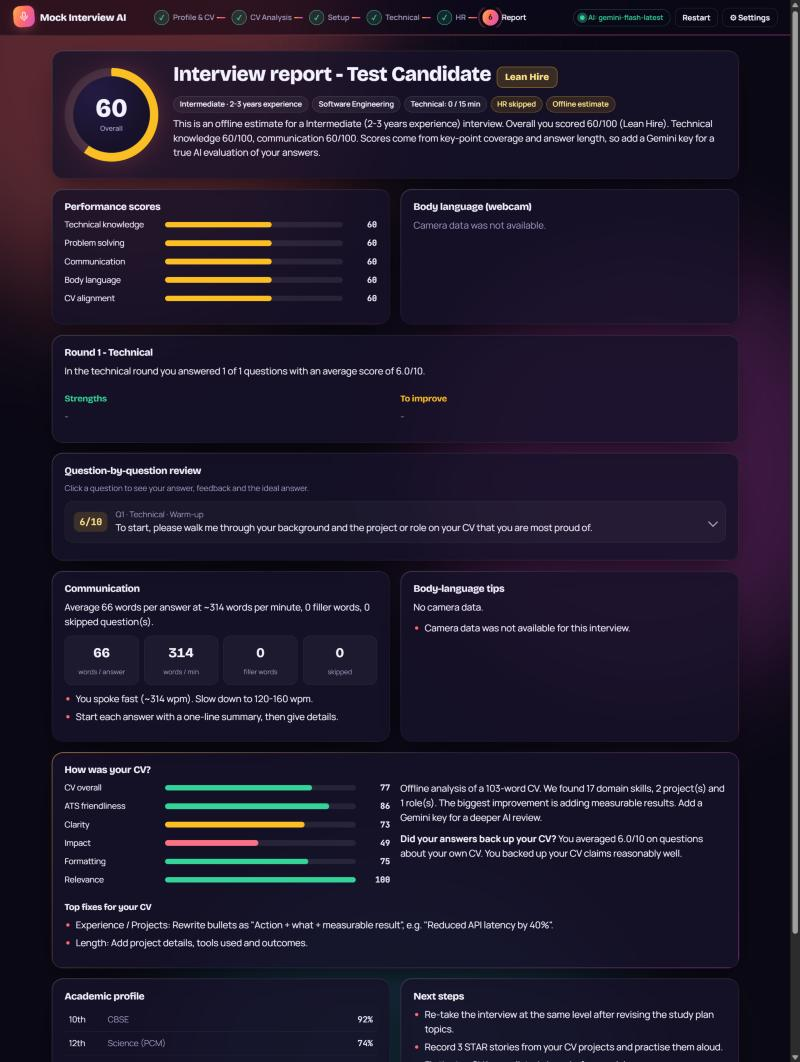
\includegraphics[width=\linewidth,height=0.78\textheight,keepaspectratio]{figures/final_report.jpg}
    \end{column}
  \end{columns}
\end{frame}

\begin{frame}{User Interface and Experience}
  \begin{columns}[T]
    \begin{column}{0.5\textwidth}
      \small
      \begin{itemize}
        \item Dark ``stage'' theme: drifting light, spotlight following the mouse, gradient accents.
        \item Motion explains state: score rings count up, bars fill, avatar pulses while speaking, questions appear word by word, listening equaliser, verdict ``stamp'', confetti for high scores.
        \item Respects the system \textbf{reduced-motion} setting.
        \item Responsive down to phone width (390 px).
      \end{itemize}
    \end{column}
    \begin{column}{0.24\textwidth}
      \centering
      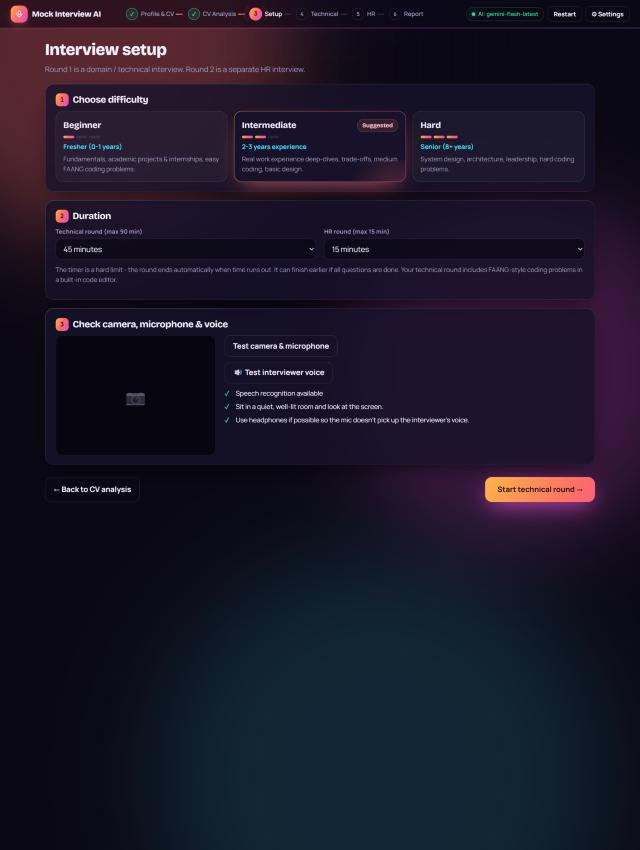
\includegraphics[width=\linewidth,height=0.78\textheight,keepaspectratio]{figures/interview_setup.jpg}
    \end{column}
    \begin{column}{0.2\textwidth}
      \centering
      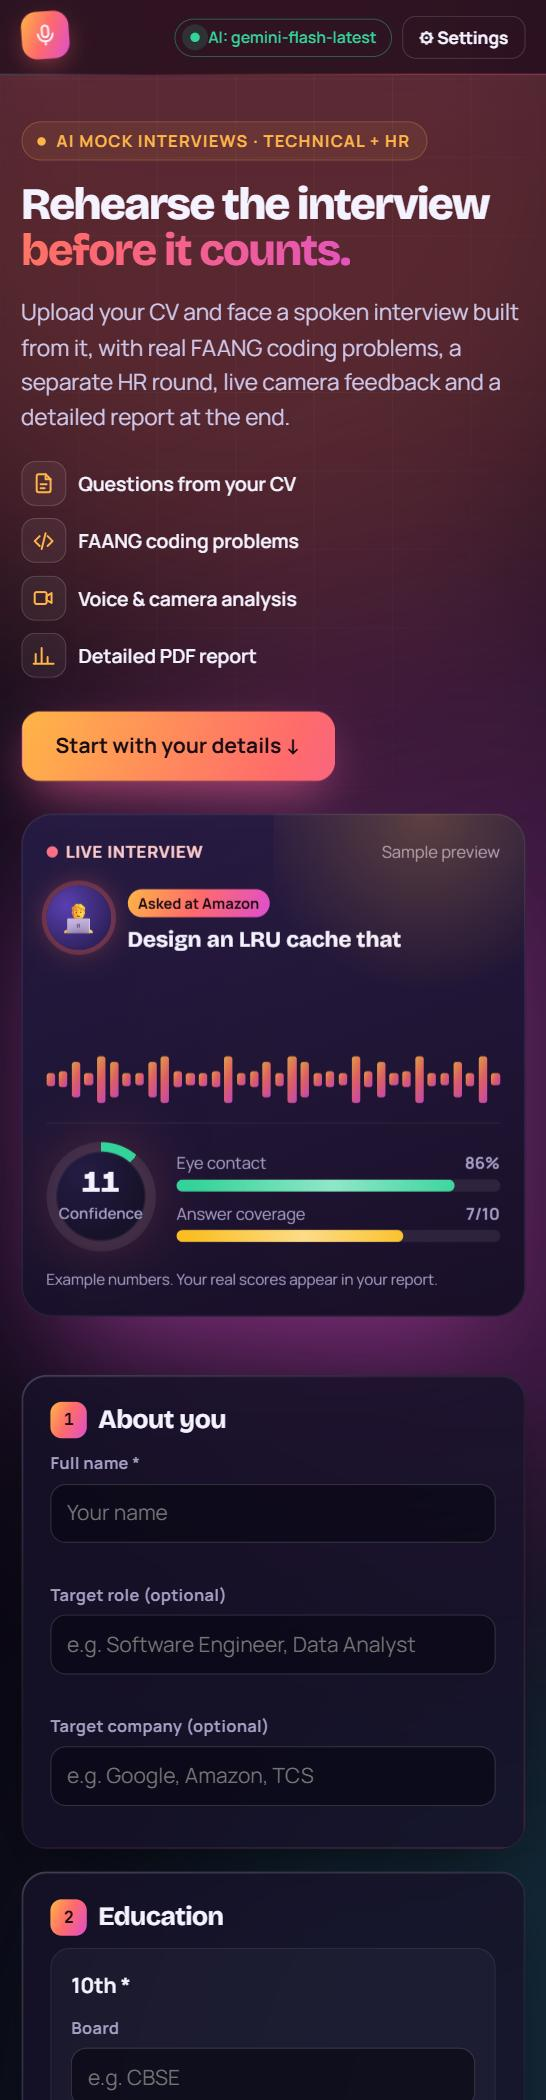
\includegraphics[width=\linewidth,height=0.78\textheight,keepaspectratio]{figures/mobile_view.jpg}
    \end{column}
  \end{columns}
\end{frame}

% =====================================================================
\section{Implementation}
\begin{frame}{Technology Stack}
  \small
  \begin{tabularx}{\textwidth}{@{}lY@{}}
    \toprule
    \textbf{Technology} & \textbf{Use} \\
    \midrule
    React 18 + Vite 5 & User interface, development server, production build \\
    Google Gemini API & CV analysis, question plans, answer evaluation, final report (JSON mode) \\
    Web Speech API & Text-to-speech (questions) and speech recognition (answers) \\
    MediaPipe Tasks Vision & Face Landmarker: landmarks + blendshapes in WebAssembly \\
    Monaco Editor & In-browser code editor \\
    pdf.js, mammoth & PDF and DOCX text extraction \\
    jsPDF & PDF report generation in the browser \\
    Netlify & Public HTTPS hosting (key-free build) \\
    \bottomrule
  \end{tabularx}
  \vspace{0.3cm}
  \begin{exampleblock}{Privacy by design}
    Video processed on the device $\cdot$ no interview history stored $\cdot$ API key never included in the public build.
  \end{exampleblock}
\end{frame}

% =====================================================================
\section{Testing and Results}
\begin{frame}{Testing}
  \footnotesize
  \begin{tabularx}{\textwidth}{@{}lYc@{}}
    \toprule
    \textbf{ID} & \textbf{Test} & \textbf{Result} \\
    \midrule
    TC01 & Complete workflow: profile $\to$ CV analysis $\to$ setup $\to$ technical $\to$ break $\to$ report & Pass \\
    TC02 & CV parsing: 21 skills, 2 projects, 2 roles; 92\% $\to$ 74\% dip flagged & Pass \\
    TC04/05 & Camera or microphone blocked: clear message, interview continues, typing works & Pass \\
    TC06 & Coding question: editor loads, code saved and scored & Pass \\
    TC07 & ``End round'' mid-answer: answer saved and scored & Pass \\
    TC10 & PDF export (multi-page file generated) & Pass \\
    TC11 & All five AI stages with a real API key & Pass \\
    TC12/13 & Model overloaded or retired: fallback; all busy: Retry / Offline shown within 77 s & Pass \\
    TC15 & Phone width 390 px: single column, no sideways scroll & Pass \\
    TC16 & Public HTTPS deployment; API key absent from all files & Pass \\
    \bottomrule
  \end{tabularx}
  \vspace{0.2cm}

  \small 17 test cases executed, all passing; 11 defects found and fixed during testing.
\end{frame}

\begin{frame}{AI Pipeline Verification (Real API Key)}
  \small
  \begin{tabularx}{\textwidth}{@{}lcYc@{}}
    \toprule
    \textbf{Stage} & \textbf{Attempts} & \textbf{Model that answered} & \textbf{Cumulative time} \\
    \midrule
    CV analysis & 1 & gemini-3.5-flash-lite & 72 s \\
    Technical question plan & 3 & gemini-3-flash-preview & 311 s \\
    Answer evaluation & 1 & gemini-3.6-flash & 339 s \\
    HR question plan & 9 & gemini-3.1-flash-lite-preview & 1111 s \\
    Final report & 1 & gemini-3.1-flash-lite-preview & 1123 s \\
    \bottomrule
  \end{tabularx}
  \vspace{0.3cm}
  \begin{itemize}
    \item 30-min plan: 6 questions, times add up to exactly 30 min, \textbf{4 of 6 from the CV}.
    \item Sample answer scored \textbf{8/10} with a relevant follow-up question.
    \item Deliberately wrong code (hash map for ``Product of Array Except Self'') detected: \textbf{2/10} with the correct prefix / suffix solution.
    \item Retries reflect service overload at test time, not application errors.
  \end{itemize}
\end{frame}

\begin{frame}{Sample Generated Questions (Intermediate, 30 min)}
  \small
  \begin{enumerate}
    \item \textbf{[CV]} Walk me through your E-Commerce Microservices Platform. Why Kafka, and how did you keep MongoDB data consistent?
    \item \textbf{[CV, asked at Amazon, Adobe]} You cut page load by 40\% with Redis. What was your cache-invalidation strategy, and how did you handle cache stampedes?
    \item \textbf{[Fundamentals]} Process vs thread, and how it changes a Node.js API vs a multi-threaded Spring Boot service.
    \item \textbf{[FAANG coding: Amazon, Meta, Apple]} Product of Array Except Self in $O(n)$ without division.
    \item \textbf{[FAANG coding]} Contains Duplicate: hash set vs sorting trade-offs.
    \item \textbf{[System design: Google, Amazon, Stripe]} Design a rate limiter for Amazon-scale API traffic.
  \end{enumerate}
  \vspace{0.2cm}
  \begin{exampleblock}{Observation}
    Questions turn CV claims into probing questions, as experienced interviewers do.
  \end{exampleblock}
\end{frame}

\begin{frame}{Results: Application Screens}
  \centering
  \begin{columns}[T]
    \begin{column}{0.32\textwidth}
      \centering
      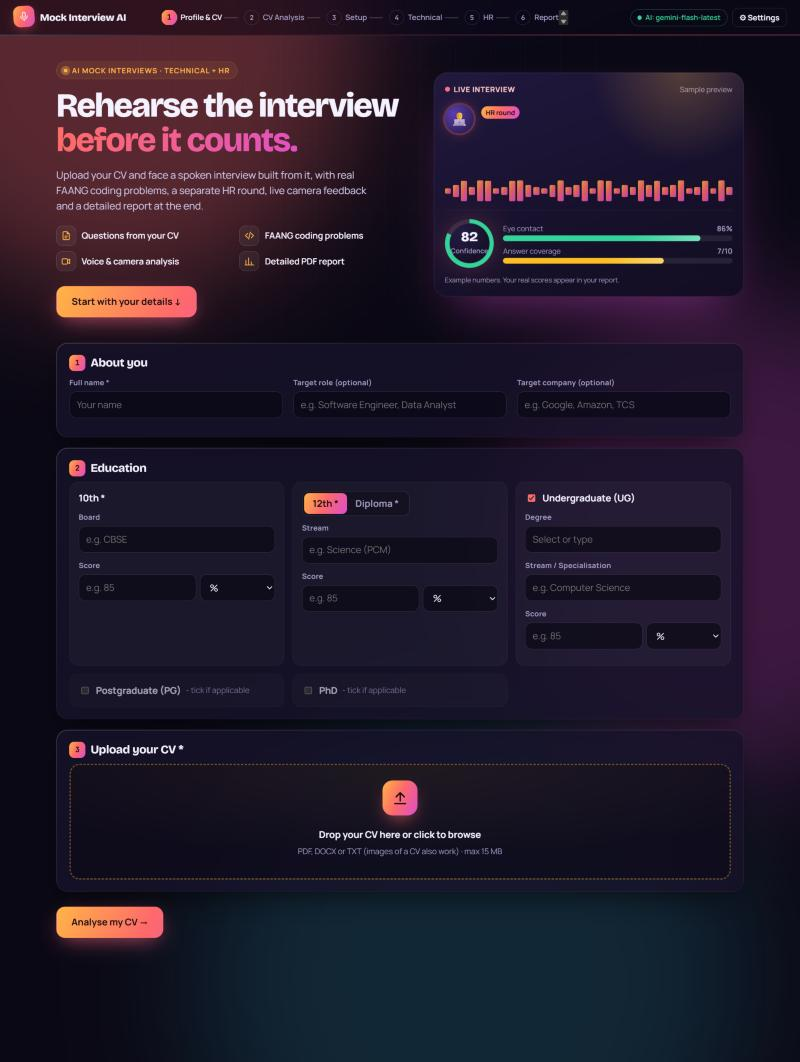
\includegraphics[width=\linewidth,height=0.62\textheight,keepaspectratio]{figures/landing_page.jpg}\\
      \scriptsize Landing and profile
    \end{column}
    \begin{column}{0.32\textwidth}
      \centering
      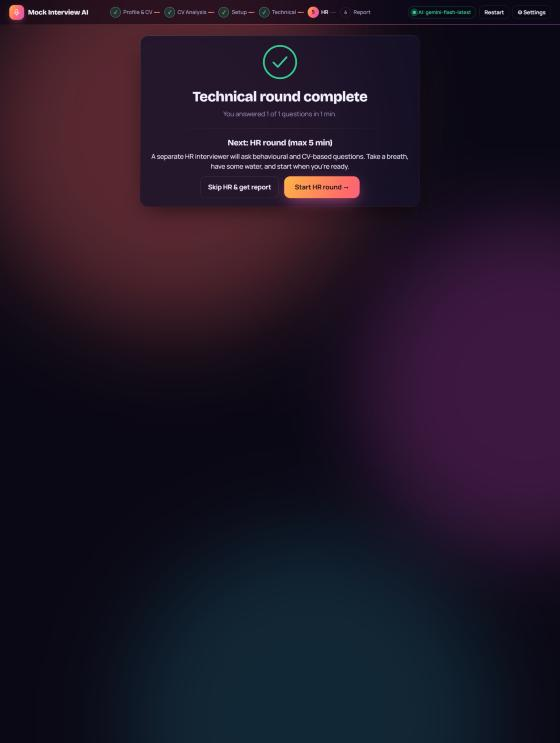
\includegraphics[width=\linewidth,height=0.62\textheight,keepaspectratio]{figures/round_break.jpg}\\
      \scriptsize Break between rounds
    \end{column}
    \begin{column}{0.32\textwidth}
      \centering
      
\includegraphics[width=\linewidth,height=0.62\textheight,keepaspectratio]{figures/loading_screen.jpg}\\
      \scriptsize Report generation
    \end{column}
  \end{columns}
\end{frame}

\begin{frame}{Defects Found and Fixed}
  \footnotesize
  \begin{tabularx}{\textwidth}{@{}YY@{}}
    \toprule
    \textbf{Defect} & \textbf{Fix} \\
    \midrule
    Answer cut off by timer / ``End round'' scored 0 & Unscored answers scored when the report is built \\
    15-min round had no CV question & At least one CV question always planned \\
    Default model retired for new keys & Auto-updating alias + fallback chain \\
    Misleading ``model not found'' when all were busy & Retired and busy models tracked separately \\
    A model could hang for 120 s & Per-request timeout + overall budget \\
    API key inside the first shareable build & Build without key file + automatic scan before upload \\
    Public site required a hosting login & Protection disabled for this site only \\
    \bottomrule
  \end{tabularx}
\end{frame}

% =====================================================================
\section{Conclusion}
\begin{frame}{Limitations}
  \begin{itemize}
    \item Speech recognition works in \textbf{Chrome and Edge}, not Firefox, and needs internet.
    \item Free AI tier: $\approx$20 requests per model per day, while a full interview uses $\approx$20; heavy use needs a paid key or Offline mode.
    \item Offline scoring is keyword-based and cannot judge the correctness of reasoning or code.
    \item Code is reviewed but \textbf{not executed} against test cases.
    \item Body-language metrics are \textbf{heuristics}, not validated against human raters; affected by lighting, camera angle and glasses.
  \end{itemize}
\end{frame}

\begin{frame}{Future Scope}
  \begin{itemize}
    \item Run submitted code against hidden test cases in a sandbox.
    \item Validate and calibrate behavioural metrics with human interviewer ratings.
    \item Prosodic analysis: pitch, volume and pauses.
    \item Interview history and progress tracking (with consent).
    \item More languages, including Indian languages.
    \item Company-specific formats and multi-interviewer panels.
    \item Desktop app with fully offline speech recognition.
  \end{itemize}
\end{frame}

\begin{frame}{Conclusion}
  \begin{itemize}
    \item Built \textbf{Mock Interview AI}: a cross-platform, browser-based, two-round mock interview.
    \item Questions come mostly from the \textbf{candidate's own CV}, plus FAANG coding problems, at three experience levels.
    \item \textbf{Spoken} questions and answers, a code editor, and \textbf{on-device} body-language analysis.
    \item Strict time limits: technical $\le 90$ min, HR $\le 15$ min.
    \item Detailed report with model answers, CV review and study plan, as \textbf{PDF}.
    \item Dependable on a free, overloaded AI service through \textbf{model fallback, quota awareness, time budgets and Offline mode}.
    \item All AI stages verified with a real key; deployed as a public HTTPS website.
  \end{itemize}
\end{frame}

\begin{frame}[allowframebreaks]{References}
  \scriptsize
  \begin{thebibliography}{10}
    \bibitem{campion1997} M.~A. Campion, D.~K. Palmer and J.~E. Campion, ``A review of structure in the selection interview,'' \emph{Personnel Psychology}, 50(3), 1997.
    \bibitem{levashina2014} J.~Levashina, C.~J. Hartwell, F.~P. Morgeson and M.~A. Campion, ``The structured employment interview,'' \emph{Personnel Psychology}, 67(1), 2014.
    \bibitem{hoque2013} M.~E. Hoque \emph{et al.}, ``MACH: My Automated Conversation coacH,'' \emph{UbiComp}, 2013.
    \bibitem{naim2018} I.~Naim, M.~I. Tanveer, D.~Gildea and M.~E. Hoque, ``Automated analysis and prediction of job interview performance,'' \emph{IEEE Trans. Affective Computing}, 9(2), 2018.
    \bibitem{lugaresi2019} C.~Lugaresi \emph{et al.}, ``MediaPipe: A framework for building perception pipelines,'' arXiv:1906.08172, 2019.
    \bibitem{kartynnik2019} Y.~Kartynnik \emph{et al.}, ``Real-time facial surface geometry from monocular video on mobile GPUs,'' \emph{CVPR Workshops}, 2019.
    \bibitem{soukupova2016} T.~Soukupov\'{a} and J.~\v{C}ech, ``Real-time eye blink detection using facial landmarks,'' \emph{CVWW}, 2016.
    \bibitem{vaswani2017} A.~Vaswani \emph{et al.}, ``Attention is all you need,'' \emph{NeurIPS}, 2017.
    \bibitem{brown2020} T.~B. Brown \emph{et al.}, ``Language models are few-shot learners,'' \emph{NeurIPS}, 2020.
    \bibitem{gemini2023} Gemini Team, Google, ``Gemini: A family of highly capable multimodal models,'' arXiv:2312.11805, 2023.
    \bibitem{zheng2023} L.~Zheng \emph{et al.}, ``Judging LLM-as-a-judge with MT-Bench and Chatbot Arena,'' \emph{NeurIPS Datasets and Benchmarks}, 2023.
    \bibitem{webspeech} W3C Audio Community Group, ``Web Speech API,'' Draft Community Group Report.
    \bibitem{mcdowell2015} G.~Laakmann McDowell, \emph{Cracking the Coding Interview}, 6th ed., CareerCup, 2015.
  \end{thebibliography}
\end{frame}

\begin{frame}[plain]
  
\begin{tikzpicture}[remember picture, overlay]
    \shade[left color=ink, right color=brandmagenta!70!ink] (current page.south west) rectangle (current page.north east);
    \fill[coral, opacity=0.25] ([xshift=-1.5cm,yshift=-1cm]current page.north east) circle (3cm);
  \end{tikzpicture}
  \vfill
  \begin{center}
    {\color{white}\Huge\bfseries Thank You\par}
    \vspace{0.4cm}
    {\color{white!85!coral}\Large Questions?\par}
    \vspace{0.8cm}
    {\color{white!80}\small Live demo: \texttt{https://mock-interview-ai-8064.netlify.app}\par}
  \end{center}
  \vfill
\end{frame}

\end{document}
